% ****** Start of file RamanCoolingV1.tex ******
%
%
% See the REVTeX 4 README file
% It also requires running BibTeX. The commands are as follows:
%
%

\documentclass[%
 reprint,
%superscriptaddress,
%groupedaddress,
%unsortedaddress,
%runinaddress,
%frontmatterverbose, 
%preprint,
%showpacs,preprintnumbers,
%nofootinbib,
%nobibnotes,
%bibnotes,
 amsmath,amssymb,
 aps,
prl,
%pra,
%prb,
%rmp,
%prstab,
%prstper,
%floatfix,
]{revtex4-1}

\usepackage{graphicx}% Include figure files
\usepackage{dcolumn}% Align table columns on decimal point
\usepackage{bm}% bold math
%\usepackage{hyperref}% add hypertext capabilities
%\usepackage[mathlines]{lineno}% Enable numbering of text and display math
%\linenumbers\relax % Commence numbering lines

%\usepackage[showframe,%Uncomment any one of the following lines to test 
%%scale=0.7, marginratio={1:1, 2:3}, ignoreall,% default settings
%%text={7in,10in},centering,
%%margin=1.5in,
%%total={6.5in,8.75in}, top=1.2in, left=0.9in, includefoot,
%%height=10in,a5paper,hmargin={3cm,0.8in},
%]{geometry}

\begin{document}

%\preprint{APS/123-QED}

\title{A Plugged Trap for Crossed Field Spin-Flip Loss}%


\author{David Reens}%
\author{Hao Wu}
\author{Tim Langen}%
\author{Jun Ye}
\affiliation{%
 Physics Department, University of Colorado at Boulder\\
}%

\date{\today}% It is always \today, today,


%%%%%%%%%%%%%%%%%%%%%
%ABSTRACT
%%%%%%%%%%%%%%%%%%%%%
\begin{abstract}
A new electromagnetic trap geometry allows tunable plugging of non-adiabatic spin flip loss in crossed electric and magnetic fields. This loss afflicts a wide set of candidate molecules and operates at much higher temperatures compared with the more familiar atomic spin-flip loss near the zero of a magnetic trap, and thus it's removal represents an important step toward ultracold molecules. Using only an external magnetic bias coil, the loss rate is tuned from over $100 \text{ s}^{-1} $ to below the vacuum limited lifetime in a $100 \text{ mK}$ sample of OH molecules.
\end{abstract}


\maketitle


%%%%%%%%%%%%%%%%%%%%%%%%%%%%%%%%%
%
%     III   NNN   TTT   RRR   OOO   DDD   UUU   CCC   TTT   III   OOO   NNN
%     III   NNN   TTT   RRR   OOO   DDD   UUU   CCC   TTT   III   OOO   NNN
%     III   NNN   TTT   RRR   OOO   DDD   UUU   CCC   TTT   III   OOO   NNN
%
%%%%%%%%%%%%%%%%%%%%%%%%%%%%%%%%%
%\section{Introduction}
The ultracold regime extends toward molecules on many fronts. Several bialkali molecules are available and others are under development. Creative and carefully engineered laser cooling strategies are tackling certain nearly rotationally diagonal molecules. A plethora of non-optical cooling strategies have succeeded to greater or lesser extents on other molecules. All of these molecules will require secondary strategies like evaporation or sympathetic cooling to make further gains in phase space density. They also may face a familiar challenge: spin flip loss near the zero of a magnetic trap, only dramatically enhancemed for certain molecules. Here we report on our encounter with OH molecule enhanced spin flip loss and our solution.

The knowledge of spin flips or Majorana hops as an eventual trap lifetime limit predates the very first magnetic trapping of neutrals\cite{Migdall1985}. Spin flips were directly observed and overcome in the TOP trap\cite{Petrich1995}, and shortly later with a plugged dipole trap\cite{Davis1995}, famously enabling the first Bose-Einstein condensates. The molecular spin-flips can occur at much higher temperatures compared with their atomic counterpart, and thus they need to be addressed much earlier than might have been expected. The magnitude of the loss varies with molecular species, and is particularly strong for the case of the neutral hydroxyl radical (OH) that we study. 

Essentially, the loss enhancement is related to the sensitivity of molecules not only to the rotation of the magnetic field in the trap, but also to the relative orientation of electric and magnetic fields. For Hund's case (a) molecules with very strong spin-rotation coupling, or for case (b) molecules to the extent that their spin-rotation coupling $\gamma$ is nonzero, electric and magnetic fields add linearly when the fields are parallel but sublinearly when the fields are orthogonal. We call this ``blocking". The presence of a constant orthogonal electric field blocks the magnetic field so that the Zeeman splitting is reduced. For ground state $^2\Pi_{3/2}$ weak field seeking OH, the Zeeman splitting is blocked from linear to cubic as shown in fig.~\ref{fig:blocking}. Since the orthogonal electric field couples opposite spin states, if these are three quanta apart as for the highest state in a $J=3/2$ manifold, the Zeeman splitting is heavily blocked from linear to cubic. This blocking means that when $B<<E$ and $B\cdot E=0$ are met, the energy gap between the highest two states is small, and spin-flips can occur. In a quadrupole trapping geometry with homogeneous electric field, these conditions are met in a plane through the origin, but not outside. This results in a worst case scenario for loss, since the energy gradients near the plane are still large, but the energy gap is small in a dramatically enhanced area of the plane, as shown in panel (e) of fig.~\ref{fig:blocking}.

\begin{figure}[b]
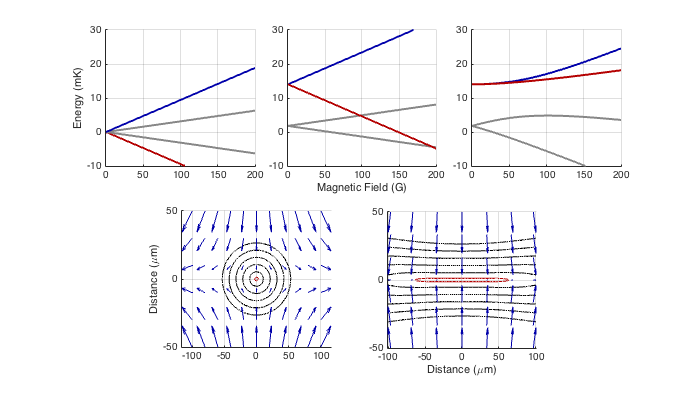
\includegraphics[width=100mm]{blocking.png}%
\caption{
The blocking effect. (a), four Zeeman split lines in the ground state of OH. A nearly identical set of four states of opposite parity lie 100 mK below. The trapped state and it's spin flip partner are in blue and red. (b) Zeeman splitting with the addition of an electric field of 150 V/cm parallel to the magnetic field. (c) Again but with the fields orthogonal. (d) Contours showing the gap between blue and red states near the zero of a magnetic quadrupole trap without electric field. (e) Again with 150 V/cm. Note the drastic widening of the lowest contour, but without gradient reduction nearby.
\label{fig:blocking}}
\end{figure}

We can apply Brillouin-Wigner perturbation theory or analytically solve the ground state eigenenergies and taylor expand to obtain the following functional form for the gap between the states where $E\cdot B=0$:

\begin{equation}
\label{eq:HZprop}
H_Z\propto \frac{B^3}{E^4}\Delta^2
\end{equation}

\noindent Here $B$, $E$, and $\Delta$ are Zeeman, Stark, and lambda doublet energies with all coefficients subsumed. We can use this to develop a scaling law for the enhancement. Let $\kappa$ be the threshold for gaps between states below which spin-flips are possible at the 50\% level. $\kappa$ depends on the velocity of trapped species, but suppose we have a specific temperature of interest, and therefore a mean velocity. Without electric field, the effective cross sectional area for a hopping region is $\pi \kappa^2$, since loss can occur where $B<\kappa$. With electric field, a much larger $B$ field is required to overcome blocking, so we have from eq.~\ref{HZprop} that $B < \sqrt[3]{\frac{\kappa E^4}{\Delta^2}}$, so for $E>\sqrt{\kappa\Delta}$ there is an enhancement given by:
\begin{equation}
\nu = \left(\frac{E^4}{\kappa^2\Delta^2}\right)^\frac{2}{3}
\label{eq:blimit}
\end{equation} 

It is interesting to note that in ref.~\cite{Lara2008}, it was specifically undertaken to investigate the spin-flip loss for OH molecules in a magnetic quadrupole trap with superposed electric field, and no enhancement was found. This turns out to be a consequence of a reasonable yet false assumption that a 4-state approximate Hamiltonian with two spin states and two parities would contain the behavior relevant for spin-flip loss in mixed fields. This approximate Hamiltonian exhibits only constant order blocking- i.e. the Zeeman effect remains linear though with adjusted slope. C.f. the gray $M_J=\pm1/2$ state curves in panel (c) of fig.~\ref{fig:blocking}.

%%%%%%%%%%%%%%%%%%%%%%%%%%
%  PIN TRAP GEOMETRY
%%%%%%%%%%%%%%%%%%%%%%%%%%


One obvious way to avoid the loss enhancement is to simply never use electric field in a magnetic trap. This prevents loss from being enhanced compared with atoms, but doesn't remove it entirely. Another possibility is to trap with electric fields, where no spin-flip loss is possible thanks to the large lambda-doublet splitting. However this splitting also results in a significant reduction in trap gradient close to the trap center, very undesirable for further cooling by evaporation, which needs as much phase space density as possible.

Seeking to remove the loss entirely but without trap gradient sacrifice, we switch from a 3D to a 2D magnetic trap, and use electric fields to trap in the remaining dimension. This does not remove the possibility of $E.B=0$, but it allows us to tune the minimum magnetic field with an external bias coil oriented along the zero axis of the 2D quadrupole trap.  Our fields are as follows:
\begin{eqnarray}
\vec{B} &=&  B^\prime y\hat{x}+ B^\prime x\hat{y} + B_{coil} \hat{z}\\
\vec{E} &=&  E^\prime y\hat{y}-  E^\prime z\hat{z}
\end{eqnarray}

\noindent In other words 2D quadrupole traps in the xy plane for B and in the yz plane for E. Serendipitously, we are able to achieve these fields with a geometry that exactly matches that of our Stark decelerator, as shown in fig.~\ref{fig:CAD}. This represents a near best-case scenario for coupling between a pulsed decelerator and a trap.

Now regarding the molecule enhanced spin-flip loss, E is perpendicular to B when:
\begin{eqnarray}
\vec{B}\cdot \vec{E} &= 0\\
B^\prime x E^\prime y - B_{coil}  E^\prime z &= 0\\
B_{coil}z &= xyB^\prime
\end{eqnarray}

So we see that E and B are perpendicular on a hyperbolic sheet which deviates more significantly from the z axis with increasing $B_{coil}$, and reduces to the pair of planes $x=0$ and $y=0$ in the limit that $B_{coil} = 0$. On this hyperbolic sheet, $B$ must be larger than the threshold set by Eq.~\ref{eq:blimit} to overcome blocking. Fortunately, $B_{coil}$ does not have to overcome the blocking limit, it only needs to push the $B\cdot E=0$ surfaces slightly away from the z-axis for the strong magnetic quadrupole fields to overcome the blocking. In fig.~\ref{fig:LSurfs}, the surfaces where $E\cdot B=0$ are colored wherever the gap there is below the threshold $\kappa$, for several different choices of $B_\text{coil}$. Since the magnetic fields are more localized than the electric, there are always regions susceptible to spin flips, but they can be pushed far enough from the trap center so as to only affect molecules which could already escape the trap by mechanical means. 

In fact, from fig.~~\ref{fig:LSurfs} it would appear that $B_{coil}$ essentially tunes the proximity of the loss regions to the trap center, and that for $B_{coil}$ large enough the loss should be removed.  

\begin{figure}[b]
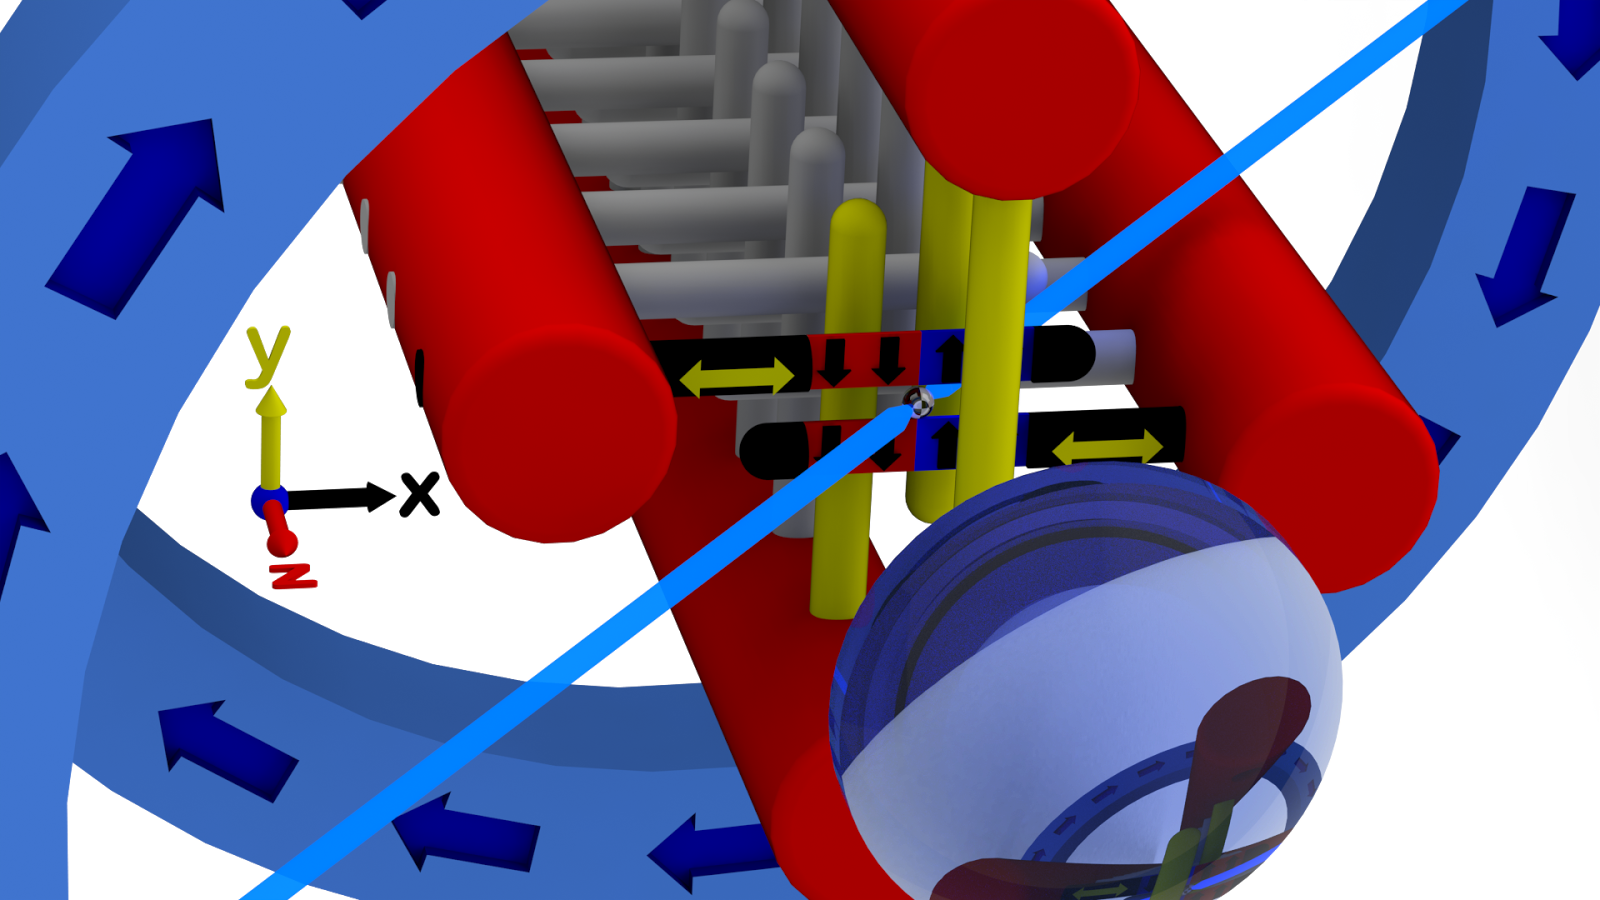
\includegraphics[width=90mm]{blue-red-yellow-v2_CAD.png}%
\caption{
OH molecules are created using a supersonic expansion source and decelerated from an initial velocity of 460m/s to a final velocity of 40ms/s using a Stark decelerator (red). The decelerator contains 142 electrode pairs (gray). Trapping is achieved by combining a radial magnetic quadrupole field, created by the magnetized second to last electrode pair of the decelerator, with a longitudinal electric quadrupole field created by the third to last and last electrode pairs, respectively (yellow, one electrode is omitted for clarity). The magnetized electrodes can be translated in situ along the x-axis to align their domains and optimize the quadrupole. As there is no trapping magnetic field in the z-direction in this configuration, macroscopic external bias coils can be used to lift the gap between the top two states of the OH ground-state manifold and thus tune the molecular loss. Detection is realized using laser induced fluorescence along the x+y-z direction (blue), which is collected using a lens system and PMT in the z-direction.
\label{fig:CAD}}
\end{figure}


\begin{figure}[b]
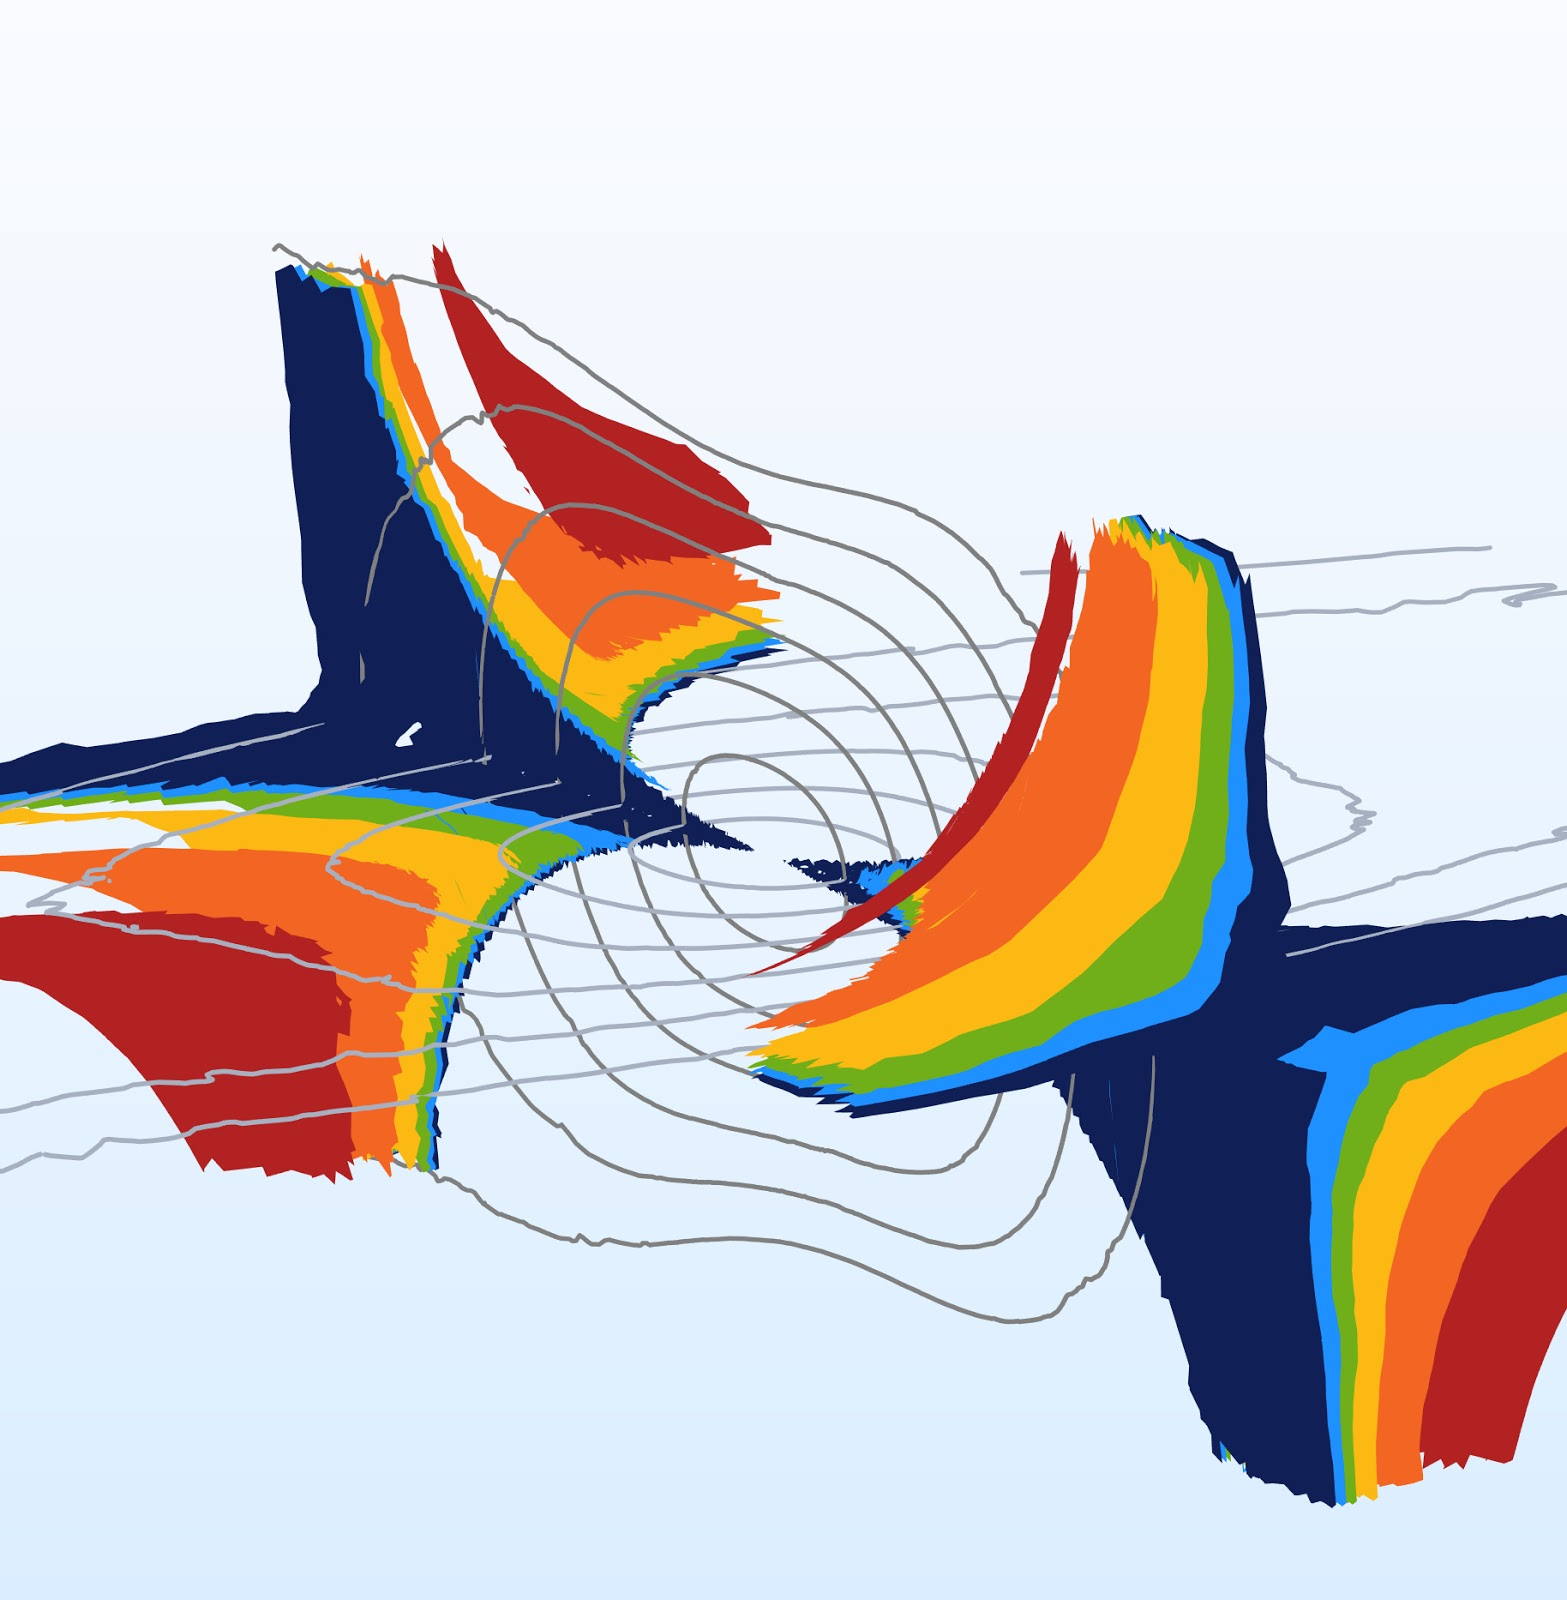
\includegraphics[width=90mm]{Loss_Surface_Chunks_0-320_0.jpeg}%
\caption{
Contours every 100mK, colors 0,20,40,80,160,320 G bias field and pin offset at zero. Molecules can spin-flip and be lost, whenever they cross these areas.
\label{fig:LSurfs}}
\end{figure}

%%%%%%%%%%%%%%%%%%%
%  LOSS TRAJECTORY DATA
%%%%%%%%%%%%%%%%%%%
\section{Loss Trajectories}
We can measure OH population in the trap as a function of time and as a function of bias field used for removing the loss. This demonstrates how truly wonderful and amazing we are.


%includes uncited bib entries
\nocite{*}


\bibliography{MolecularMajoranaLoss.bib}% Produces the bibliography via BibTeX.

\end{document}
%
% ****** End of file MolecularMajoranaLoss.tex ******
